\documentclass[10pt]{article}
\usepackage[a4paper, margin=2cm]{geometry}
%\usepackage{fullpage}
\usepackage[T1]{fontenc}
\usepackage[utf8]{inputenc}
\usepackage{hyperref}
\hypersetup{
    colorlinks=true,      
    urlcolor=blue
    }
\usepackage{graphicx}
\usepackage{mathpazo}
\pagenumbering{arabic}
\usepackage{siunitx}
\usepackage{amsmath}
\usepackage{mathtools} % Para poder usar "\Aboxed"
\usepackage{cancel} % Para usar "\cancel", de https://tex.stackexchange.com/questions/537955/how-do-cross-out-text-in-math-mode
\usepackage{multicol}
\usepackage[spanish]{babel}
\usepackage{steinmetz}
\DeclareSIUnit\voltampere{VA}
\DeclareSIUnit\var{VAr}
\setlength\parindent{0pt} % no indent

% Numbering pages on the right footer:
% (https://tex.stackexchange.com/questions/153167/how-to-set-page-number-at-right-footer)
\usepackage{fancyhdr}
% Turn on the style
\pagestyle{fancy}
\fancyhf{} % sets both header and footer to nothing
\renewcommand{\headrulewidth}{0pt} % To remove the top horizontal line created by default by "fancyhdr", from here: https://tex.stackexchange.com/questions/13896/how-to-remove-the-top-horizontal-bar-in-fancyhdr
% Set the right side of the footer to be the page number
\fancyfoot[R]{\thepage}


\usepackage{minibox} % Para poder partir el texto en 2 líneas usando "underbrace" u "overbrace", info aquí: https://tex.stackexchange.com/questions/8680/how-can-i-insert-a-newline-in-a-framebox


\usepackage{xparse} % For "overbrace/underbrace but with an arrow instead", from https://tex.stackexchange.com/questions/8720/overbrace-underbrace-but-with-an-arrow-instead

% Para poner flechas sobre los signos de igual, de aquí: https://tex.stackexchange.com/questions/8720/overbrace-underbrace-but-with-an-arrow-instead
\NewDocumentCommand{\overarrow}{O{=} O{\uparrow} m}{%
  \overset{\makebox[0pt]{\begin{tabular}{@{}c@{}}#3\\[0pt]\ensuremath{#2}\end{tabular}}}{#1}
}
\NewDocumentCommand{\underarrow}{O{=} O{\downarrow} m}{%
  \underset{\makebox[0pt]{\begin{tabular}{@{}c@{}}\ensuremath{#2}\\[0pt]#3\end{tabular}}}{#1}
}





\begin{document}

\large{\textbf{Ejemplo 1.13} del \href{https://raw.githubusercontent.com/ETSIDI-IE/tc/master/docs/TC.pdf}{libro de la asignatura}} 

\vspace{3mm}
\large{\textbf{Enunciado}}:

\vspace{3mm}
En el circuito de la figura se debe emplear el método de los nudos para determinar:

\vspace{1mm}            
\begin{enumerate}
    \item Las tensiones en los nudos $A$ y $B$
    \item Las corrientes de rama señaladas
    \item El balance de potencias, diferenciando entre elementos activos y elementos pasivos
\end{enumerate}

\vspace{3mm}

\begin{minipage}{0.78\linewidth}
  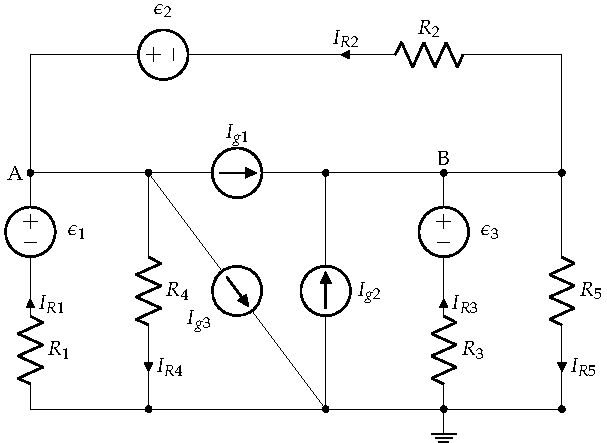
\includegraphics[scale=1.2]{figs/nudos_fuentes.pdf}
\end{minipage}
\begin{minipage}{0.20\linewidth}
    \textbf{Datos}:
    \vspace{2mm}
    
    $R_1 = R_3 = R_4 = $\\
    $ \hspace*{12mm} = R_5 = \qty{2}{\ohm}$\\ 
    $R_2 = \qty{1}{\ohm}$\\
    $\epsilon_1=\qty{6}{\volt}$\\
    $\epsilon_2 = \qty{12}{\volt}$\\
    $\epsilon_3 = \qty{24}{\volt}$\\
    $I_{g_1} = \qty{15}{\ampere}$\\
    $I_{g_2} = \qty{9}{\ampere}$\\
    $I_{g_3} = \qty{6}{\ampere}$
\end{minipage}

\vspace{7mm}

\hrulefill

\vspace{8mm}
\textbf{Solución}:
\vspace{4mm}

En el circuito hay tres fuentes de tensión en serie con resistencias, que se deben transformar en fuentes de corriente para poder aplicar el método de nudos:

\begin{align*}
    I_{\epsilon_1}&=\dfrac{\epsilon_1}{R_1}=\dfrac{6}{2}=3\,\text{A}\\
    I_{\epsilon_2}&=\dfrac{\epsilon_2}{R_2}=\dfrac{12}{1}=12\,\text{A}\\
    I_{\epsilon_3}&=\dfrac{\epsilon_3}{R_3}=\dfrac{24}{2}=12\,\text{A}\\
\end{align*}

\vspace{-2mm}
\begin{center}
    (esquema del circuito transformado en la siguiente página)
\end{center}

\begin{center}
    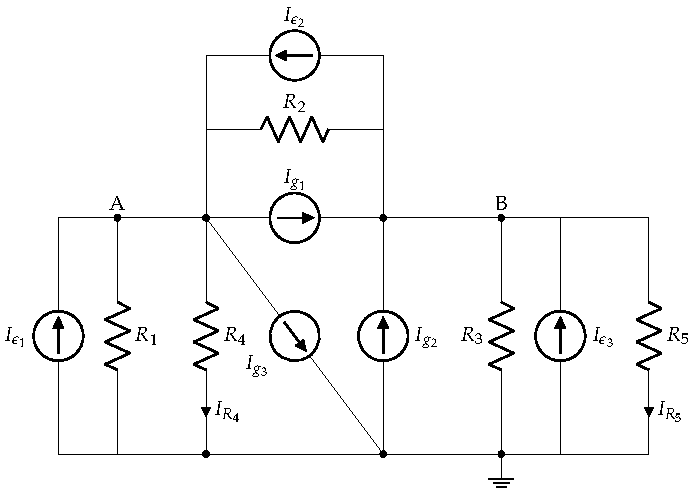
\includegraphics[scale=1.2]{figs/nudos_fuentes2.pdf}
\end{center}

\vspace{2mm}
Aplicamos ahora la ecuación general de método de los nudos al circuito, que consta únicamente de 2 nudos independientes:

\begin{equation*}
    \begin{bmatrix}
      \dfrac{1}{2}+\dfrac{1}{2}+\dfrac{1}{1} & -\dfrac{1}{1}\\[10pt]
      -\dfrac{1}{1} & \dfrac{1}{1}+\dfrac{1}{2}+\dfrac{1}{2}
    \end{bmatrix}
    \cdot
    \begin{bmatrix}
      \vphantom{\dfrac{1}{1}} U_A\\[10pt]
      \vphantom{\dfrac{1}{1}} U_B
    \end{bmatrix}
    =
    \begin{bmatrix}
      \vphantom{\dfrac{1}{1}} 3+12-15-6\\[10pt]
      \vphantom{\dfrac{1}{1}} 15+9+12-12
    \end{bmatrix}
\end{equation*}

\vspace{5mm}
Cuya solución es:

\vspace{-6mm}
\begin{align*}
    \Aboxed{U_A &= \qty{4}{\volt}}\\
    \Aboxed{U_B &= \qty{14}{\volt}}
\end{align*}

\vspace{4mm}
A partir de las tensiones, se determinan las corrientes de rama señaladas, aplicando 2LK:
\begin{align*}
  U_A = \epsilon_1-I_{R_1}\cdot R_1 
  \quad &\Rightarrow \quad 
  I_{R_1} = \dfrac{6-4}{2} = \Aboxed{\qty{1}{\ampere}}\\
  U_{AB} = U_A - U_B = -10 = \epsilon_2 - I_{R_2}\cdot R_2 
  \quad &\Rightarrow \quad 
  I_{R_2} = \dfrac{12-(-10)}{1} = \Aboxed{\qty{22}{\ampere}}\\
  U_B = \epsilon_3 - I_{R_3}\cdot R_3 
  \quad &\Rightarrow \quad 
  I_{R_3} = \dfrac{24-14}{2} = \Aboxed{\qty{5}{\ampere}}\\
  &\qquad\;\; I_{R_4} = \dfrac{U_A}{R_4} = \dfrac{4}{2} = \Aboxed{\qty{2}{\ampere}}\\
  &\qquad\;\; I_{R_5} = \dfrac{U_B}{R_5} = \dfrac{14}{2} = \Aboxed{\qty{7}{\ampere}}
\end{align*}

\vspace{2mm}
\emph{Se recomienda comprobar que estos resultados cumplen la 1LK} en cada uno de los 2 nudos independientes del \underline{circuito original} (antes de transformar las fuentes de tensión, porque tambien podríais haber cometido errores al transformar las fuentes), para asegurarse de que la resolución es correcta.

Ya tenemos toda la información necesaria para formular el balance de potencias pedido en el último apartado:

\begin{itemize}
\item \textbf{Potencia de los generadores:}
  \begin{align*}
    \qquad\qquad\qquad\qquad\qquad\qquad P_{Ig_1} &= I_1 \cdot U_{BA} = \qty{150}{\watt}\\
    P_{Ig_2} &= I_2 \cdot U_{B} = \qty{126}{\watt}\\
    P_{Ig_3} &= I_3 \cdot (-U_{A}) = - \qty{24}{\watt} \quad \text{(se comporta como receptor)}\\
    P_{\epsilon_1} &= \epsilon_1 \cdot I_{R_1} = \qty{6}{\watt}\\
    P_{\epsilon_2} &= \epsilon_2 \cdot I_{R_2} = \qty{264}{\watt}\\
    P_{\epsilon_3} &= \epsilon_3 \cdot I_{R_3} = \qty{120}{\watt}
  \end{align*}
  Los elementos activos aportan un total de \qty{642}{\watt}.
\item \textbf{Potencia de las resistencias:}
  \begin{align*}
    P_{R_1} &= (I_{R_1})^2 \cdot R_1 = \qty{2}{\watt}\\
    P_{R_2} &= (I_{R_2})^2 \cdot R_2 = \qty{484}{\watt}\\
    P_{R_3} &= (I_{R_3})^2 \cdot R_3 = \qty{50}{\watt}\\
    P_{R_4} &= (I_{R_4})^2 \cdot R_4 = \qty{8}{\watt}\\
    P_{R_5} &= (I_{R_5})^2 \cdot R_5 = \qty{98}{\watt}
  \end{align*}
  Las resistencias disipan un total de \SI{642}{\watt}.
\end{itemize}

Comprobamos que la potencia total entregada por los generadores es igual a la potencia total consumida por las resistencias.

\end{document}
